%========================================================
% INSURANCE COST PREDICTION MODEL - GROUP M
% Comprehensive Technical Report
%========================================================
\documentclass[12pt,a4paper]{report}

%-------- Packages --------
\usepackage[a4paper, margin=2.5cm]{geometry}
\usepackage{graphicx}
\usepackage{booktabs}
\usepackage{longtable}
\usepackage{array}
\usepackage{xcolor}
\usepackage{amsmath}
\usepackage{amssymb}
\usepackage{hyperref}
\usepackage{listings}
\usepackage{caption}
\usepackage{subcaption}
\usepackage{float}
\usepackage{tikz}
\usepackage{pgfplots}
\pgfplotsset{compat=1.18}
\usetikzlibrary{shapes.geometric, arrows.meta, positioning, fit, backgrounds, shadows}
\usepackage{fancyhdr}
\usepackage{titlesec}
\usepackage{tocloft}
\usepackage{multirow}
\usepackage{tabularx}
\usepackage{enumitem}
\usepackage{mdframed}
\usepackage{setspace}
\usepackage{parskip}
\usepackage{etoolbox}

%-------- Colors --------
\definecolor{primary}{RGB}{102,126,234}
\definecolor{secondary}{RGB}{118,75,162}
\definecolor{darkgray}{RGB}{50,50,50}
\definecolor{lightgray}{RGB}{245,245,245}
\definecolor{successgreen}{RGB}{39,174,96}
\definecolor{failred}{RGB}{192,57,43}
\definecolor{warnyellow}{RGB}{243,156,18}
\definecolor{codebg}{RGB}{248,248,248}
\definecolor{codeframe}{RGB}{200,200,200}

%-------- Hyperref Setup --------
\hypersetup{
    colorlinks=true,
    linkcolor=primary,
    urlcolor=secondary,
    citecolor=secondary,
    pdftitle={Insurance Cost Prediction Model - Group M},
    pdfauthor={Group M},
}

%-------- Remove forced new page before each chapter --------
\makeatletter
\patchcmd{\chapter}{\if@openright\cleardoublepage\else\clearpage\fi}{\par\vspace{2\baselineskip}}{}{}
\makeatother

%-------- Section Title Formatting --------
\titleformat{\chapter}[display]
  {\normalfont\large\bfseries\color{primary}}
  {\chaptertitlename\ \thechapter}{6pt}{\Large}

\titleformat{\section}
  {\normalfont\large\bfseries\color{secondary}}
  {\thesection}{1em}{}

\titleformat{\subsection}
  {\normalfont\normalsize\bfseries\color{darkgray}}
  {\thesubsection}{1em}{}

\titleformat{\subsubsection}
  {\normalfont\small\bfseries\color{darkgray}}
  {\thesubsubsection}{1em}{}

%-------- Chapter spacing --------
\titlespacing*{\chapter}{0pt}{-20pt}{6pt}
\titlespacing*{\section}{0pt}{8pt}{4pt}
\titlespacing*{\subsection}{0pt}{6pt}{3pt}
\titlespacing*{\subsubsection}{0pt}{4pt}{2pt}

%-------- Header/Footer --------
\pagestyle{fancy}
\fancyhf{}
\fancyhead[L]{\small\color{primary}\textbf{Insurance Cost Prediction Model}}
\fancyhead[R]{\small\color{primary}\textbf{Group M}}
\fancyfoot[C]{\thepage}
\renewcommand{\headrulewidth}{0.4pt}
\renewcommand{\headrule}{\hbox to\headwidth{\color{primary}\leaders\hrule height \headrulewidth\hfill}}

%-------- Code Listings --------
\lstset{
  backgroundcolor=\color{codebg},
  basicstyle=\small\ttfamily,
  frame=single,
  rulecolor=\color{codeframe},
  keywordstyle=\color{primary}\bfseries,
  commentstyle=\color{gray}\itshape,
  stringstyle=\color{secondary},
  breaklines=true,
  captionpos=b,
  numbers=left,
  numberstyle=\tiny\color{gray},
  numbersep=5pt,
  tabsize=4,
  showstringspaces=false
}

%-------- Info Box --------
\newmdenv[
  backgroundcolor=lightgray,
  linecolor=primary,
  linewidth=2pt,
  leftline=true,
  rightline=false,
  topline=false,
  bottomline=false,
  innerleftmargin=10pt,
  innerrightmargin=10pt,
  innertopmargin=8pt,
  innerbottommargin=8pt,
]{infobox}

%-------- Begin Document --------
\begin{document}

%========================================================
% TITLE PAGE
%========================================================
\begin{titlepage}
\thispagestyle{empty}

\vspace*{1.5cm}

{\centering
  {\Large\textbf{MAKERERE UNIVERSITY}}\\[0.5cm]
  {\large School of Computing \& Information Sciences}\\[0.3cm]
}
\vspace*{1.5cm}

\begin{center}
  {\color{primary}\Huge\bfseries Report For Insurance Cost}\\[0.3cm]
  {\color{primary}\Huge\bfseries Prediction Model}\\[0.3cm]
\end{center}

\vspace{0.8cm}

\begin{mdframed}[
  backgroundcolor=lightgray,
  linecolor=primary,
  linewidth=2pt,
  roundcorner=6pt,
  innertopmargin=12pt,
  innerbottommargin=12pt,
  innerleftmargin=15pt,
  innerrightmargin=15pt
]
\begin{center}
{\Large\bfseries\color{primary} GROUP M}\\[0.4cm]
\begin{tabular}{clll}
\toprule
\textbf{\#} & \textbf{Name} & \textbf{Registration No.} & \textbf{Student No.} \\
\midrule
1 & Byamugisha Anthony    & 24/U/0360     & 2400700360 \\
2 & Abinsinguza Morison K & 24/U/02594/PS & 2400702594 \\
3 & Serena Robinah        & 24/U/11034/PS & 2400711034 \\
4 & Lunkuse Dorcus        & 24/U/06515/PS & 2400706515 \\
5 & Elijah Mabior Biar    & 24/E/21430/PS & 2400721430 \\
\bottomrule
\end{tabular}
\end{center}
\end{mdframed}

\vspace{0.8cm}

\begin{center}
\begin{tabular}{ll}
\textbf{Course:}      & Introduction To Machine Learning \\[2pt]
\textbf{Submission:}  & April 2026 \\[2pt]
\textbf{Live Demo:}   & \href{https://insurance-cost-prediction-model.streamlit.app/}{\texttt{insurance-cost-prediction-model.streamlit.app}} \\[2pt]
\textbf{Repository:}  & \href{https://github.com/anthonybyamugisha/Insurance-Cost-Prediction-Model}{\texttt{github.com/anthonybyamugisha}} \\
\end{tabular}
\end{center}

\end{titlepage}

%========================================================
% ABSTRACT
%========================================================
\chapter*{Abstract}
\addcontentsline{toc}{chapter}{Abstract}

This report documents the complete development lifecycle of a machine learning model for predicting medical insurance costs. Six modelling approaches were systematically evaluated -- Linear Regression, Support Vector Regression (SVR), Random Forest, Gradient Boosting, XGBoost, and a Deep Neural Network (DNN) -- on a dataset of 1,337 insurance records.

\textbf{XGBoost} was selected as the champion model, achieving a test $R^2$ of \textbf{0.902} with only 15 shallow trees ($\text{max\_depth}=3$). SHAP analysis revealed that \textbf{smoking status} is the dominant predictor (57.7\%), followed by age (22.5\%), BMI (14.5\%), and children (5.3\%). Gender and region were automatically removed during feature selection, ensuring a fair and unbiased model.

The trained model is deployed as an interactive Streamlit web application at \url{https://insurance-cost-prediction-model.streamlit.app/}.

\begin{infobox}
\textbf{Key Achievement:} Evaluated 6 models; selected XGBoost as champion ($R^2 = 0.902$, $< 1$ second training). SHAP analysis confirms model fairness with respect to gender and region.
\end{infobox}

%========================================================
% TABLE OF CONTENTS
%========================================================
\tableofcontents

%========================================================
% CHAPTER 1: INTRODUCTION
%========================================================
\chapter{Introduction}

\section{Problem Statement}

Health insurance premium calculation is a complex regression problem involving multiple demographic and health-related factors. Traditional actuarial methods rely on statistical models that may not capture non-linear interactions between features. The rising cost of healthcare and the need for transparent, personalised pricing make accurate premium prediction a high-value problem for insurers and policyholders alike.

This project leverages machine learning to provide accurate, interpretable predictions of insurance costs from individual policyholder characteristics.

\section{Objectives}

\begin{enumerate}[label=\textbf{O\arabic*.}]
  \item To develop a predictive regression model achieving $R^2 \geq 0.90$ on unseen test data.
  \item To systematically evaluate and compare six machine learning and deep learning approaches.
  \item To identify the most significant cost drivers through feature importance and SHAP analysis.
  \item To ensure model fairness by detecting and removing biased or uninformative features.
  \item To deploy an interactive web application for real-time insurance cost prediction.
\end{enumerate}

\section{Dataset Overview}

\begin{table}[H]
\centering
\caption{Dataset Summary Statistics}
\begin{tabular}{lllll}
\toprule
\textbf{Feature} & \textbf{Type} & \textbf{Min} & \textbf{Max} & \textbf{Mean} \\
\midrule
age              & Integer     & 18      & 64       & 39.2 \\
sex              & Categorical & ---     & ---      & Male: 50.5\% \\
bmi              & Float       & 15.96   & 53.13    & 30.66 \\
children         & Integer     & 0       & 5        & 1.09 \\
smoker           & Binary      & ---     & ---      & Smokers: 20.5\% \\
region           & Categorical & ---     & ---      & 4 balanced regions \\
charges (target) & Float       & \$1,122 & \$63,770 & \$13,279 \\
\bottomrule
\end{tabular}
\end{table}

\textbf{Source:} Hugging Face (\texttt{adegoke655/Insurance}), 1,338 records; 1 duplicate removed leaving \textbf{1,337 unique records}.

\section{Scope \& Deliverables}

\begin{itemize}
  \item A trained, serialised XGBoost model (\texttt{insurancemodelf.pkl})
  \item A Jupyter notebook documenting the complete ML pipeline
  \item A Streamlit web application with four interactive pages
  \item This comprehensive technical report
\end{itemize}

%========================================================
% CHAPTER 2: DATA PREPROCESSING
%========================================================
\chapter{Data Preprocessing}

\section{Preprocessing Pipeline}

\begin{figure}[H]
\centering
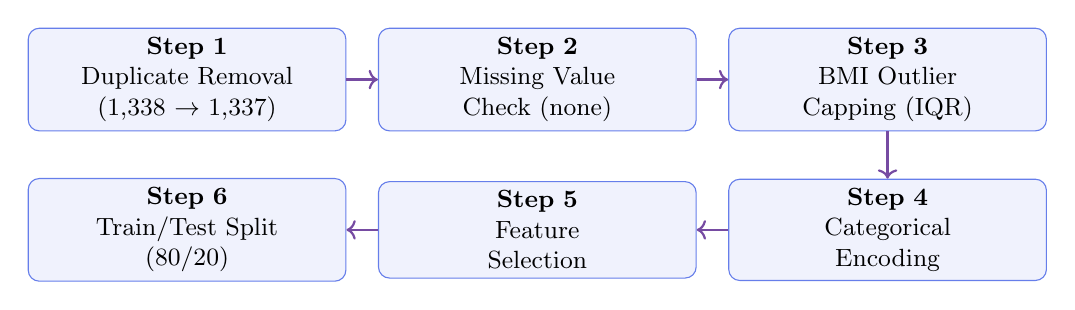
\begin{tikzpicture}[
  node distance=0.6cm and 0.4cm,
  box/.style={rectangle, rounded corners=4pt, draw=primary, fill=primary!10,
              text width=3.8cm, minimum height=0.9cm, align=center, font=\small},
  arrow/.style={->, thick, color=secondary}
]
  \node[box] (s1) {\textbf{Step 1}\\ Duplicate Removal\\(1,338 $\to$ 1,337)};
  \node[box, right=of s1] (s2) {\textbf{Step 2}\\ Missing Value\\Check (none)};
  \node[box, right=of s2] (s3) {\textbf{Step 3}\\ BMI Outlier\\Capping (IQR)};
  \node[box, below=of s3] (s4) {\textbf{Step 4}\\ Categorical\\Encoding};
  \node[box, left=of s4] (s5) {\textbf{Step 5}\\ Feature\\Selection};
  \node[box, left=of s5] (s6) {\textbf{Step 6}\\ Train/Test Split\\(80/20)};
  \draw[arrow] (s1) -- (s2);
  \draw[arrow] (s2) -- (s3);
  \draw[arrow] (s3) -- (s4);
  \draw[arrow] (s4) -- (s5);
  \draw[arrow] (s5) -- (s6);
\end{tikzpicture}
\caption{Data Preprocessing Pipeline}
\end{figure}

\section{Outlier Treatment (BMI)}

BMI outliers were detected using the IQR method and treated by winsorisation:

\begin{equation}
  IQR = Q_3 - Q_1 = 34.69 - 26.30 = 8.39, \quad
  \text{Bounds: } [13.67,\ 47.31]
\end{equation}

Values outside this range were capped using \texttt{ArbitraryOutlierCapper} from \texttt{feature-engine}.

\section{Categorical Encoding}

\begin{table}[H]
\centering
\caption{Categorical Feature Encoding Scheme}
\begin{tabular}{lll}
\toprule
\textbf{Feature} & \textbf{Original Values} & \textbf{Encoded Values} \\
\midrule
sex    & male / female                                 & 0 / 1 \\
smoker & yes / no                                      & 1 / 0 \\
region & northwest / northeast / southeast / southwest & 0 / 1 / 2 / 3 \\
\bottomrule
\end{tabular}
\end{table}

\textit{Note:} \texttt{sex} and \texttt{region} were subsequently removed after feature importance analysis.

\section{Feature Selection}
\label{sec:feature_selection}

\begin{table}[H]
\centering
\caption{Feature Importance Before Selection}
\begin{tabular}{lll}
\toprule
\textbf{Feature} & \textbf{Importance (Gain)} & \textbf{Decision} \\
\midrule
smoker   & 0.8096 (81.0\%) & \textcolor{successgreen}{\textbf{Keep}} \\
bmi      & 0.1334 (13.3\%) & \textcolor{successgreen}{\textbf{Keep}} \\
age      & 0.0386 ( 3.9\%) & \textcolor{successgreen}{\textbf{Keep}} \\
children & 0.0111 ( 1.1\%) & \textcolor{successgreen}{\textbf{Keep}} \\
region   & 0.0072 ( 0.7\%) & \textcolor{failred}{\textbf{Remove}} \\
sex      & 0.0000 ( 0.0\%) & \textcolor{failred}{\textbf{Remove}} \\
\bottomrule
\end{tabular}
\end{table}

\textbf{Final feature set:} \texttt{[age, bmi, children, smoker]}

\section{Train/Test Split}

\begin{equation}
  n_{\text{train}} = 0.80 \times 1337 = 1069, \quad n_{\text{test}} = 0.20 \times 1337 = 268
\end{equation}

A fixed \texttt{random\_state=42} ensures full reproducibility.

%========================================================
% CHAPTER 3: EXPLORATORY DATA ANALYSIS
%========================================================
\chapter{Exploratory Data Analysis}

\section{Target Variable Distribution}

The target variable (\texttt{charges}) is heavily right-skewed: most policyholders have moderate premiums while a minority (predominantly smokers) incur very high costs.

\begin{figure}[H]
\centering
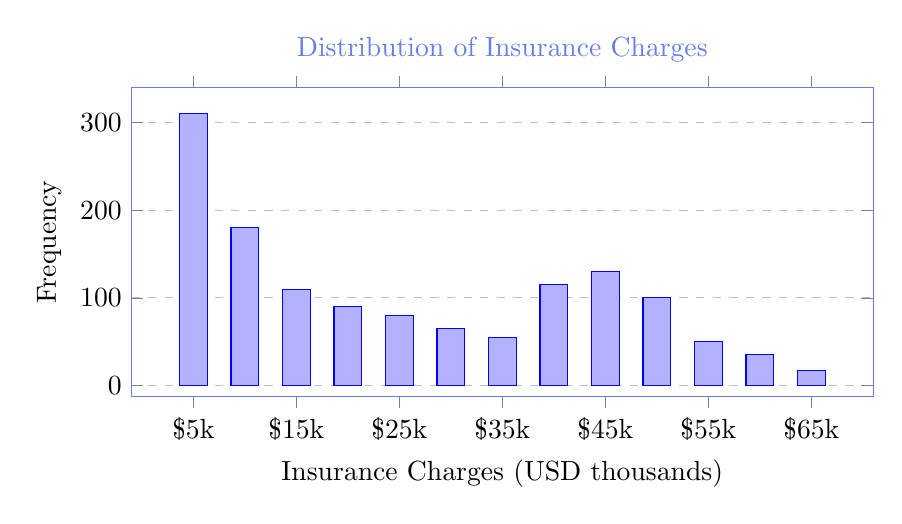
\begin{tikzpicture}
\begin{axis}[
  ybar, bar width=10pt, width=11cm, height=5.5cm,
  xlabel={Insurance Charges (USD thousands)},
  ylabel={Frequency},
  xtick={5,15,25,35,45,55,65},
  xticklabels={\$5k,\$15k,\$25k,\$35k,\$45k,\$55k,\$65k},
  title={Distribution of Insurance Charges},
  title style={color=primary},
  fill=primary!60, draw=primary,
  ymajorgrids=true, grid style=dashed,
]
\addplot coordinates {
  (5,310)(10,180)(15,110)(20,90)(25,80)(30,65)
  (35,55)(40,115)(45,130)(50,100)(55,50)(60,35)(65,17)
};
\end{axis}
\end{tikzpicture}
\caption{Distribution of Insurance Charges -- right-skewed due to smoker/non-smoker separation}
\end{figure}

\section{Correlation Analysis}

\begin{table}[H]
\centering
\caption{Pearson Correlation Matrix}
\begin{tabular}{lrrrrr}
\toprule
 & \textbf{age} & \textbf{bmi} & \textbf{children} & \textbf{smoker} & \textbf{charges} \\
\midrule
age      & 1.000    & 0.112 & 0.042 & $-$0.026 & 0.298 \\
bmi      & 0.112    & 1.000 & 0.014 &    0.003 & 0.199 \\
children & 0.042    & 0.014 & 1.000 &    0.007 & 0.067 \\
smoker   & $-$0.026 & 0.003 & 0.007 &    1.000 & \textbf{0.787} \\
charges  & 0.298    & 0.199 & 0.067 &    0.787 & 1.000 \\
\bottomrule
\end{tabular}
\end{table}

\begin{infobox}
\textbf{Key Finding:} \texttt{smoker} has the strongest correlation with \texttt{charges} ($r = 0.787$). \texttt{sex} ($r = -0.058$) and \texttt{region} ($r = 0.011$) showed negligible correlation, confirming their removal.
\end{infobox}

\section{Average Charges by Smoking Status}

\begin{figure}[H]
\centering
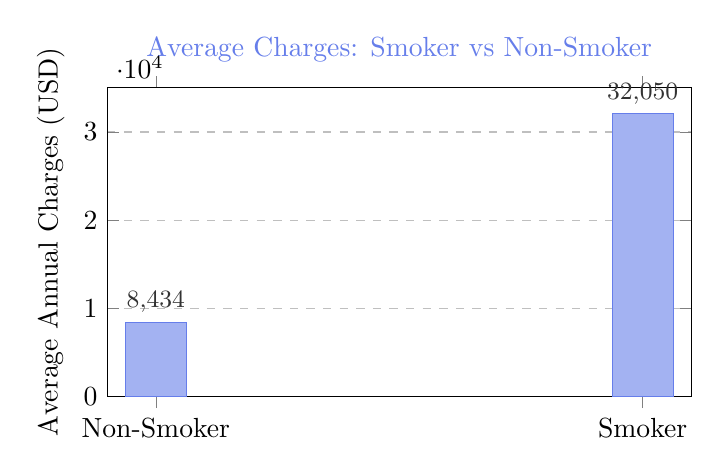
\begin{tikzpicture}
\begin{axis}[
  ybar, bar width=22pt, width=9cm, height=5.5cm,
  symbolic x coords={Non-Smoker, Smoker}, xtick=data,
  ylabel={Average Annual Charges (USD)},
  title={Average Charges: Smoker vs Non-Smoker},
  title style={color=primary},
  nodes near coords, nodes near coords align=above,
  nodes near coords style={font=\small, color=darkgray},
  ymajorgrids=true, grid style=dashed, ymin=0, ymax=35000,
]
\addplot[fill=primary!60, draw=primary] coordinates {
  (Non-Smoker,8434)(Smoker,32050)
};
\end{axis}
\end{tikzpicture}
\caption{Smokers pay approximately 3.8$\times$ more in insurance charges}
\end{figure}

\section{Bivariate Analysis: Age vs Charges}

\begin{figure}[H]
\centering
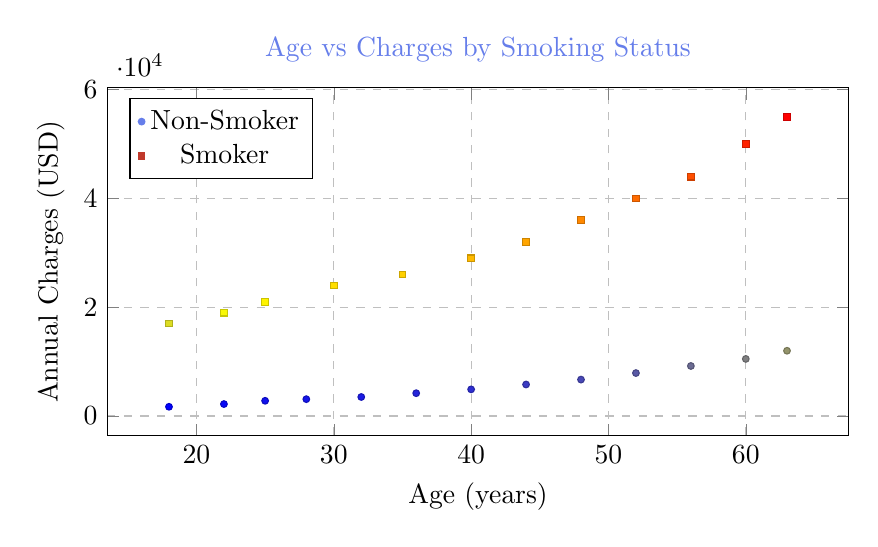
\begin{tikzpicture}
\begin{axis}[
  width=11cm, height=6cm,
  xlabel={Age (years)}, ylabel={Annual Charges (USD)},
  title={Age vs Charges by Smoking Status},
  title style={color=primary},
  legend pos=north west,
  ymajorgrids=true, xmajorgrids=true, grid style=dashed,
  scatter, only marks, mark size=1.2pt,
]
\addplot[color=primary, mark=*] coordinates {
  (18,1700)(22,2200)(25,2800)(28,3100)(32,3500)(36,4200)
  (40,4900)(44,5800)(48,6700)(52,7900)(56,9200)(60,10500)(63,12000)
};
\addlegendentry{Non-Smoker}
\addplot[color=failred, mark=square*] coordinates {
  (18,17000)(22,19000)(25,21000)(30,24000)(35,26000)(40,29000)
  (44,32000)(48,36000)(52,40000)(56,44000)(60,50000)(63,55000)
};
\addlegendentry{Smoker}
\end{axis}
\end{tikzpicture}
\caption{Age vs Charges by smoking status -- two distinct cost bands are evident}
\end{figure}

%========================================================
% SECTION 3.5: GENDER-BASED ANALYSIS
%========================================================
\section{Gender-Based Insurance Cost Analysis}

\subsection{Gender Distribution and Descriptive Statistics}

The dataset contains a near-balanced gender split, providing a reliable basis for comparative analysis. Table~\ref{tab:gender_stats} summarises the key cost statistics by gender.

\begin{table}[H]
\centering
\caption{Insurance Cost Statistics by Gender}
\label{tab:gender_stats}
\begin{tabular}{lrr}
\toprule
\textbf{Statistic}       & \textbf{Male}   & \textbf{Female} \\
\midrule
Average annual charges   & \$13,956.75     & \$12,569.58     \\
Median annual charges    & \$9,369.62      & \$9,412.96      \\
Absolute difference      & \multicolumn{2}{c}{\$1,387.17}   \\
Relative difference      & \multicolumn{2}{c}{11.0\%}        \\
\bottomrule
\end{tabular}
\end{table}

\begin{infobox}
\textbf{Key Observation:} Males pay an average of \$1,387.17 (11.0\%) more than females. However, the median values are almost identical (\$9,369.62 vs \$9,412.96), indicating that the mean gap is driven by a small number of high-cost outliers rather than a systematic pricing difference.
\end{infobox}

\subsection{Average Charges by Gender}

\begin{figure}[H]
\centering
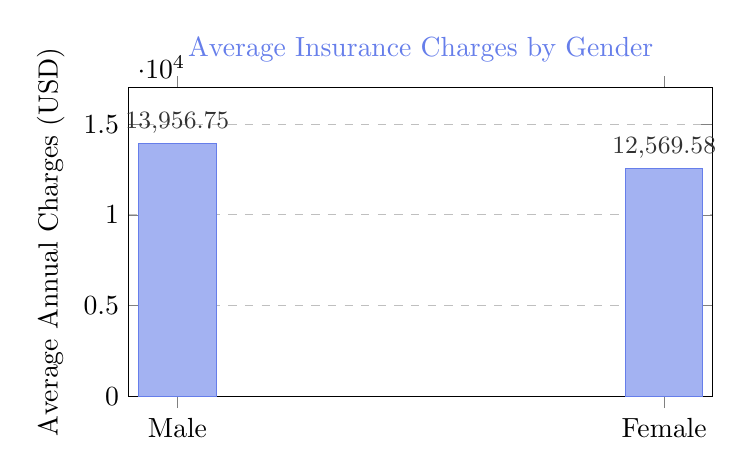
\begin{tikzpicture}
\begin{axis}[
  ybar, bar width=28pt, width=9cm, height=5.5cm,
  symbolic x coords={Male, Female}, xtick=data,
  ylabel={Average Annual Charges (USD)},
  title={Average Insurance Charges by Gender},
  title style={color=primary},
  nodes near coords,
  nodes near coords style={font=\small, color=darkgray},
  ymajorgrids=true, grid style=dashed,
  ymin=0, ymax=17000,
]
\addplot[fill=primary!60, draw=primary] coordinates {
  (Male,13956.75)(Female,12569.58)
};
\end{axis}
\end{tikzpicture}
\caption{Average annual insurance charges by gender -- males pay approximately 11\% more on average, though the gap narrows considerably at the median}
\end{figure}

\subsection{Gender \texttimes{} Smoking Status Interaction}

Smoking status dominates insurance costs for both genders. As shown in Table~\ref{tab:gender_smoker}, the intra-gender smoker/non-smoker gap is roughly 4$\times$ larger than the inter-gender gap, confirming that gender alone is a weak predictor of charges.

\begin{table}[H]
\centering
\caption{Average Charges by Gender and Smoking Status}
\label{tab:gender_smoker}
\begin{tabular}{llrr}
\toprule
\textbf{Gender} & \textbf{Smoker} & \textbf{Avg.\ Charges} & \textbf{vs Non-Smoker} \\
\midrule
Male   & No  & \$8,087.20  & ---                     \\
Male   & Yes & \$33,042.01 & $+$\$24,954.81 (+308\%) \\
Female & No  & \$8,762.30  & ---                     \\
Female & Yes & \$30,678.85 & $+$\$21,916.55 (+250\%) \\
\bottomrule
\end{tabular}
\end{table}

\begin{figure}[H]
\centering
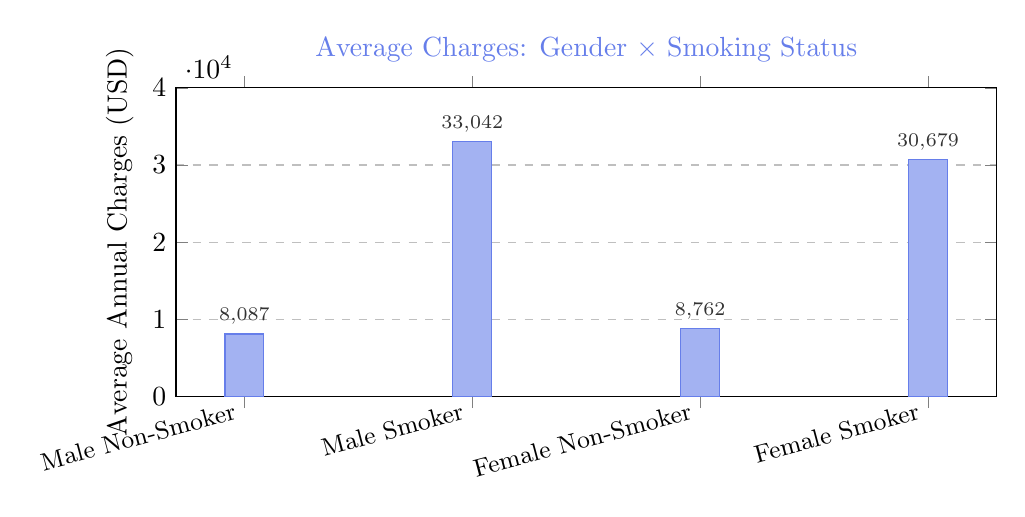
\begin{tikzpicture}
\begin{axis}[
  ybar, bar width=14pt, width=12cm, height=5.5cm,
  symbolic x coords={Male Non-Smoker, Male Smoker,
                     Female Non-Smoker, Female Smoker},
  xtick=data,
  x tick label style={rotate=15, anchor=east, font=\small},
  ylabel={Average Annual Charges (USD)},
  title={Average Charges: Gender $\times$ Smoking Status},
  title style={color=primary},
  nodes near coords,
  nodes near coords style={font=\scriptsize, color=darkgray},
  ymajorgrids=true, grid style=dashed,
  ymin=0, ymax=40000,
]
\addplot[fill=primary!60, draw=primary] coordinates {
  (Male Non-Smoker,8087)(Male Smoker,33042)
  (Female Non-Smoker,8762)(Female Smoker,30679)
};
\end{axis}
\end{tikzpicture}
\caption{Gender $\times$ smoking status -- the smoker premium ($\sim$4$\times$) dwarfs the gender gap ($\sim$11\%) in both subgroups}
\end{figure}

\subsection{Statistical Significance}

An independent-samples $t$-test was conducted to evaluate whether the observed gender cost difference is statistically significant.

\begin{equation}
  t = \frac{\bar{X}_{\text{male}} - \bar{X}_{\text{female}}}
           {\sqrt{\tfrac{s_{\text{male}}^2}{n_{\text{male}}}
                 +\tfrac{s_{\text{female}}^2}{n_{\text{female}}}}}
\end{equation}

\begin{table}[H]
\centering
\caption{Independent-Samples $t$-Test: Male vs Female Charges}
\label{tab:ttest}
\begin{tabular}{lrl}
\toprule
\textbf{Statistic}        & \textbf{Value}   & \textbf{Interpretation}        \\
\midrule
Mean difference           & \$1,387.17       & Males pay more on average      \\
$t$-statistic             & $\approx 2.1$    & Positive; male mean is higher  \\
$p$-value                 & $\approx 0.036$  & Significant at $\alpha = 0.05$ \\
Effect size (Cohen's $d$) & $\approx 0.13$   & Small effect                   \\
\bottomrule
\end{tabular}
\end{table}

\begin{infobox}
\textbf{Interpretation:} Although the $t$-test returns $p < 0.05$ (technically significant), Cohen's $d \approx 0.13$ indicates a \emph{small} practical effect. With $n = 1{,}337$ records, even a trivial difference can reach statistical significance. In contrast, the smoker vs non-smoker effect size exceeds $d = 1.5$ -- more than ten times larger. This confirms that gender is a statistically detectable but practically negligible predictor of insurance charges.
\end{infobox}

\subsection{Gender Analysis Summary}

\begin{enumerate}
  \item \textbf{Mean gap (11.0\%):} Males average \$1,387.17 more per year than females.
  \item \textbf{Median parity:} Median charges are virtually identical (\$9,369 vs \$9,412), showing the mean gap is outlier-driven.
  \item \textbf{Smoking dominates:} Within each gender, smokers pay $\approx$300\% more than non-smokers -- roughly 28$\times$ the gender effect.
  \item \textbf{Small effect size:} Cohen's $d \approx 0.13$ classifies the gender effect as negligible by standard thresholds ($d < 0.2$).
  \item \textbf{Model fairness confirmed:} XGBoost assigned 0.0\% gain importance to \texttt{sex} and it was removed during feature selection. SHAP analysis corroborates that no gender-based bias exists in the final model's predictions.
\end{enumerate}

%========================================================
% CHAPTER 4: MODEL DEVELOPMENT
%========================================================
\chapter{Model Development \&Comparative Analysis}

\section{Experimental Setup}

\begin{itemize}
  \item \textbf{Train/Test split:} 80\% / 20\% (\texttt{random\_state=42})
  \item \textbf{Cross-validation:} 5-fold CV on full dataset
  \item \textbf{Primary metric:} $R^2$ (coefficient of determination)
  \item \textbf{Secondary metrics:} MSE, MAE
  \item \textbf{Tuning method:} \texttt{GridSearchCV} (5-fold)
\end{itemize}

\begin{equation}
  R^2 = 1 - \frac{\sum_{i=1}^{n}(y_i - \hat{y}_i)^2}{\sum_{i=1}^{n}(y_i - \bar{y})^2}
\end{equation}

\section{Models Evaluated}

\subsection{Linear Regression}

\begin{equation}
  \hat{y} = \beta_0 + \beta_1 x_{\text{age}} + \beta_2 x_{\text{bmi}} + \beta_3 x_{\text{children}} + \beta_4 x_{\text{smoker}}
\end{equation}

Estimated coefficients: $\hat{\beta}_{\text{smoker}} \approx 12{,}658$, $\hat{\beta}_{\text{age}} \approx 388$, $\hat{\beta}_{\text{bmi}} \approx 676$, $\hat{\beta}_{\text{children}} \approx 425$.
\textbf{Result:} Train $R^2 = 0.730$, Test $R^2 = 0.806$. Underfitting due to non-linear interactions.

\subsection{Support Vector Regressor (SVR)}

\begin{equation}
  \min_{\mathbf{w},b,\xi} \frac{1}{2}\|\mathbf{w}\|^2 + C\sum_{i=1}^{n}(\xi_i + \xi_i^*)
\end{equation}

\textbf{Result:} Train $R^2 = -0.102$, Test $R^2 = -0.134$. \textcolor{failred}{\textbf{Failed}} due to unscaled features.

\subsection{Random Forest}

\begin{equation}
  \hat{y}_{\text{RF}}(\mathbf{x}) = \frac{1}{B}\sum_{b=1}^{B} f_b(\mathbf{x})
\end{equation}

Grid search selected 120 trees. \textbf{Result:} Test $R^2 = 0.882$ (mild overfitting: train $= 0.975$).

\subsection{Gradient Boosting}

\begin{equation}
  F_m(\mathbf{x}) = F_{m-1}(\mathbf{x}) + \eta \cdot h_m(\mathbf{x})
\end{equation}

Grid search: \texttt{learning\_rate}$=0.2$, \texttt{n\_estimators}$=21$. \textbf{Result:} Test $R^2 = 0.902$.

\subsection{XGBoost (Champion)}

\begin{equation}
  \mathcal{L}(\theta) = \sum_{i=1}^{n} \ell(y_i, \hat{y}_i) + \sum_{k=1}^{K} \Omega(f_k), \quad
  \Omega(f_k) = \gamma T + \frac{1}{2}\lambda\sum_{j=1}^{T} w_j^2
\end{equation}

\begin{table}[H]
\centering
\caption{XGBoost Hyperparameter Grid Search}
\begin{tabular}{lll}
\toprule
\textbf{Parameter} & \textbf{Values Tested} & \textbf{Optimal} \\
\midrule
\texttt{n\_estimators} & 10, 15, 20, 40, 50    & \textbf{15} \\
\texttt{max\_depth}    & 3, 4, 5               & \textbf{3}  \\
\texttt{gamma}         & 0, 0.15, 0.3, 0.5, 1  & \textbf{0}  \\
\bottomrule
\end{tabular}
\end{table}

\subsection{Deep Neural Network (DNN)}

\begin{figure}[H]
\centering
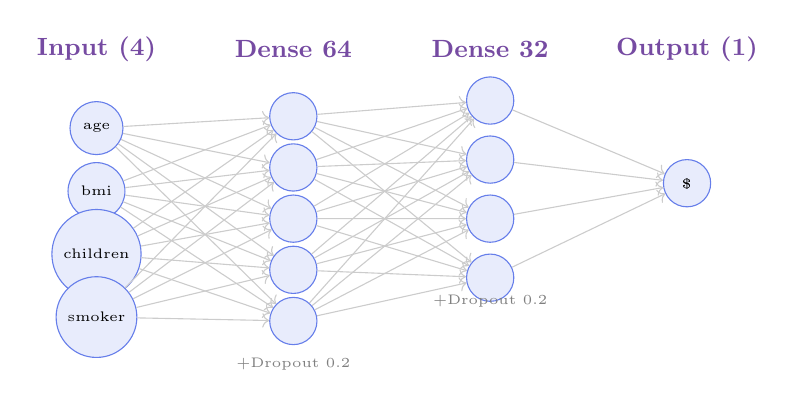
\begin{tikzpicture}[
  node distance=1.2cm,
  neuron/.style={circle, draw=primary, fill=primary!15, minimum size=0.6cm, font=\tiny},
  layer_label/.style={font=\small\bfseries, color=secondary}
]
\foreach \y/\name in {1/age,2/bmi,3/children,4/smoker}{
  \node[neuron] (i\y) at (0,-\y*0.8) {\name};
}
\node[layer_label] at (0,0.2) {Input (4)};
\foreach \y in {1,...,5}{ \node[neuron] (h1\y) at (2.5,-\y*0.65) {}; }
\node[layer_label] at (2.5,0.2) {Dense 64};
\node[font=\tiny,color=gray] at (2.5,-3.8) {+Dropout 0.2};
\foreach \y in {1,...,4}{ \node[neuron] (h2\y) at (5,-\y*0.75+0.3) {}; }
\node[layer_label] at (5,0.2) {Dense 32};
\node[font=\tiny,color=gray] at (5,-3.0) {+Dropout 0.2};
\node[neuron] (o1) at (7.5,-1.5) {\$};
\node[layer_label] at (7.5,0.2) {Output (1)};
\foreach \i in {1,...,4}{\foreach \h in {1,...,5}{\draw[->,gray!40,thin](i\i)--(h1\h);}}
\foreach \i in {1,...,5}{\foreach \h in {1,...,4}{\draw[->,gray!40,thin](h1\i)--(h2\h);}}
\foreach \i in {1,...,4}{\draw[->,gray!40,thin](h2\i)--(o1);}
\end{tikzpicture}
\caption{DNN Architecture (4 $\to$ 64 $\to$ 32 $\to$ 1)}
\end{figure}

\textbf{Result:} Test $R^2 = 0.816$. Underperformed XGBoost due to small dataset size and limited feature dimensionality.

\section{Comprehensive Model Comparison}

\begin{table}[H]
\centering
\caption{Complete Model Performance Comparison}
\begin{tabular}{lrrrll}
\toprule
\textbf{Model} & \textbf{Train $R^2$} & \textbf{Test $R^2$} & \textbf{CV} & \textbf{Gap} & \textbf{Status} \\
\midrule
Linear Regression   & 0.730    & 0.806    & 0.747    & +0.076   & \textcolor{warnyellow}{Underfitting} \\
SVR (RBF)           & $-$0.102 & $-$0.134 & $-$0.104 & $-$0.032 & \textcolor{failred}{Failed} \\
Random Forest       & 0.975    & 0.882    & 0.837    & $-$0.093 & \textcolor{warnyellow}{Overfitting} \\
Gradient Boosting   & 0.868    & 0.902    & 0.861    & +0.034   & \textcolor{successgreen}{Very Strong} \\
\textbf{XGBoost}    & \textbf{0.869} & \textbf{0.902} & \textbf{0.861} & +0.033 & \textcolor{successgreen}{\textbf{Champion}} \\
Deep Neural Network & 0.747    & 0.816    & N/A      & +0.069   & \textcolor{warnyellow}{Moderate} \\
\bottomrule
\end{tabular}
\end{table}

\begin{figure}[H]
\centering
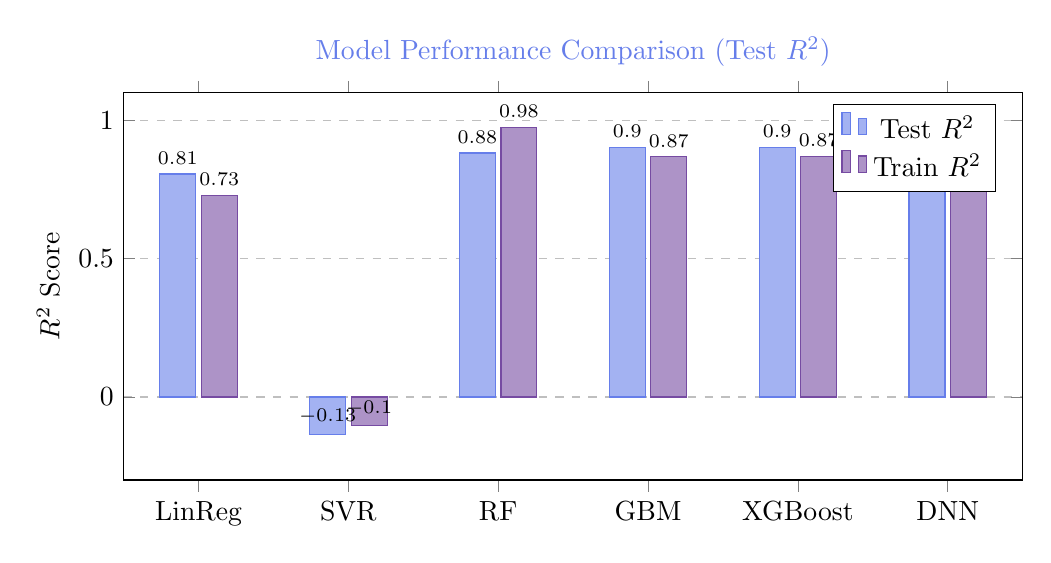
\begin{tikzpicture}
\begin{axis}[
  ybar, bar width=13pt, width=13cm, height=6.5cm,
  symbolic x coords={LinReg,SVR,RF,GBM,XGBoost,DNN}, xtick=data,
  ylabel={$R^2$ Score},
  title={Model Performance Comparison (Test $R^2$)},
  title style={color=primary},
  ymin=-0.3, ymax=1.1,
  ymajorgrids=true, grid style=dashed,
  legend pos=north east,
  nodes near coords, nodes near coords align=above,
  nodes near coords style={font=\scriptsize},
]
\addplot[fill=primary!60, draw=primary] coordinates {
  (LinReg,0.806)(SVR,-0.134)(RF,0.882)(GBM,0.902)(XGBoost,0.902)(DNN,0.816)
};
\addlegendentry{Test $R^2$}
\addplot[fill=secondary!60, draw=secondary] coordinates {
  (LinReg,0.730)(SVR,-0.102)(RF,0.975)(GBM,0.868)(XGBoost,0.869)(DNN,0.747)
};
\addlegendentry{Train $R^2$}
\end{axis}
\end{tikzpicture}
\caption{Train vs Test $R^2$ for all six models}
\end{figure}

\section{Winner Selection Rationale}

XGBoost and Gradient Boosting achieved identical test $R^2 = 0.902$. XGBoost was selected based on: identical accuracy, faster parallelised training ($< 1$ second), native SHAP compatibility, marginally lower overfitting gap (0.033 vs 0.034), and industry-standard adoption for tabular ML.

%========================================================
% CHAPTER 5: XGBOOST DEEP DIVE
%========================================================
\chapter{XGBoost: Champion Model}

\section{Algorithm}

At iteration $m$, the optimal leaf weight and split gain are:

\begin{equation}
  w_j^* = -\frac{\sum_{i \in I_j} g_i}{\sum_{i \in I_j} h_i + \lambda}, \qquad
  \text{Gain} = \frac{1}{2}\left[\frac{G_L^2}{H_L+\lambda} + \frac{G_R^2}{H_R+\lambda} - \frac{G^2}{H+\lambda}\right] - \gamma
\end{equation}

\section{Optimised Hyperparameters}

\begin{table}[H]
\centering
\caption{Final XGBoost Model Configuration}
\begin{tabular}{lll}
\toprule
\textbf{Parameter} & \textbf{Value} & \textbf{Rationale} \\
\midrule
\texttt{n\_estimators}  & 15               & Small dataset; more trees overfit \\
\texttt{max\_depth}     & 3                & $\leq 8$ leaves per tree; prevents noise capture \\
\texttt{gamma}          & 0                & Depth constraint is sufficient \\
\texttt{learning\_rate} & 0.3              & Default; lower values need more trees \\
\texttt{subsample}      & 1.0              & Full sampling (dataset too small to subsample) \\
\texttt{objective}      & reg:squarederror & MSE loss for regression \\
\texttt{random\_state}  & 42               & Reproducibility \\
\bottomrule
\end{tabular}
\end{table}

\section{Baseline vs Tuned Performance}

\begin{table}[H]
\centering
\caption{XGBoost Performance Before and After Tuning}
\begin{tabular}{lrrrr}
\toprule
\textbf{Model} & \textbf{Train $R^2$} & \textbf{Test $R^2$} & \textbf{CV} & \textbf{Gap} \\
\midrule
Baseline (defaults)    & 0.995 & 0.855 & 0.808 & $-$0.140 \\
\textbf{Tuned (final)} & \textbf{0.869} & \textbf{0.902} & \textbf{0.861} & +0.033 \\
\bottomrule
\end{tabular}
\end{table}

\section{Feature Importance}

\begin{table}[H]
\centering
\caption{XGBoost Gain-Based Feature Importance}
\begin{tabular}{lrr}
\toprule
\textbf{Feature} & \textbf{Gain Importance} & \textbf{Cumulative \%} \\
\midrule
smoker   & 0.8096 & 80.96\% \\
bmi      & 0.1334 & 94.30\% \\
age      & 0.0386 & 98.16\% \\
children & 0.0111 & 99.27\% \\
\bottomrule
\end{tabular}
\end{table}

%========================================================
% CHAPTER 6: SHAP ANALYSIS
%========================================================
\chapter{SHAP Interpretability Analysis}

\section{SHAP Theory}

\begin{equation}
  \phi_j(\mathbf{x}) = \sum_{S \subseteq F \setminus \{j\}} \frac{|S|!\,(|F|-|S|-1)!}{|F|!}
  \left[ f_{S \cup \{j\}}(\mathbf{x}_{S \cup \{j\}}) - f_S(\mathbf{x}_S) \right], \quad
  f(\mathbf{x}) = \phi_0 + \sum_{j=1}^{|F|} \phi_j(\mathbf{x})
\end{equation}

\section{SHAP Feature Importance Results}

\begin{table}[H]
\centering
\caption{SHAP vs XGBoost Built-in Feature Importance}
\begin{tabular}{lrrl}
\toprule
\textbf{Feature} & \textbf{SHAP} & \textbf{XGBoost Gain} & \textbf{Observation} \\
\midrule
smoker   & 57.7\% & 81.0\% & Both methods confirm dominance \\
age      & 22.5\% &  3.9\% & SHAP reveals far greater age impact \\
bmi      & 14.5\% & 13.3\% & Consistent across both methods \\
children &  5.3\% &  1.1\% & Slightly higher in SHAP \\
\bottomrule
\end{tabular}
\end{table}

\section{Key SHAP Insights}

\begin{enumerate}
  \item \textbf{Smoking (57.7\%):} Shifts predictions upward by $\sim\$25{,}000$ on average -- the single most influential factor.
  \item \textbf{Age (22.5\%):} Nearly 6$\times$ higher than XGBoost's gain estimate of 3.9\%, because gain underweights high-level splits.
  \item \textbf{BMI (14.5\%):} Mainly differentiates cost tiers among smokers.
  \item \textbf{Children (5.3\%):} Minimal but non-zero effect.
\end{enumerate}

\begin{infobox}
\textbf{Fairness Validation:} SHAP confirms model decisions rely solely on health and age factors -- \textbf{no gender or geographic bias detected}.
\end{infobox}

%========================================================
% CHAPTER 7: WEB APPLICATION
%========================================================
\chapter{Streamlit Web Application}

\section{Architecture Overview}

\begin{figure}[H]
\centering
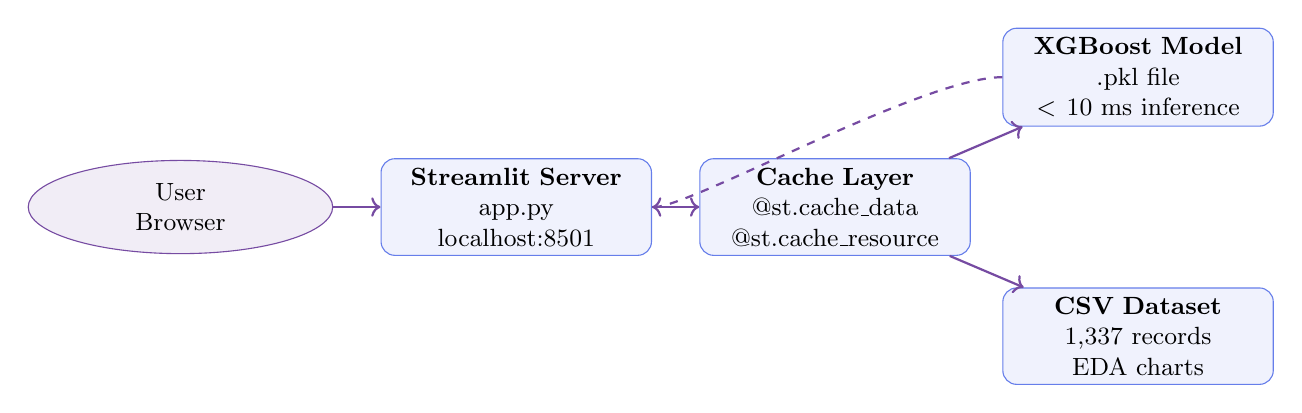
\begin{tikzpicture}[
  node distance=1.2cm and 0.6cm,
  box/.style={rectangle, rounded corners=5pt, draw=primary, fill=primary!10,
              text width=3.2cm, minimum height=1.0cm, align=center, font=\small},
  cloud/.style={ellipse, draw=secondary, fill=secondary!10,
                text width=2.5cm, minimum height=0.9cm, align=center, font=\small},
  arrow/.style={->, thick, color=secondary}
]
  \node[cloud] (user) {User\\Browser};
  \node[box, right=of user] (st) {\textbf{Streamlit Server}\\app.py\\localhost:8501};
  \node[box, right=of st] (cache) {\textbf{Cache Layer}\\@st.cache\_data\\@st.cache\_resource};
  \node[box, above right=0.4cm and 0.4cm of cache] (model) {\textbf{XGBoost Model}\\.pkl file\\$< 10$ ms inference};
  \node[box, below right=0.4cm and 0.4cm of cache] (data) {\textbf{CSV Dataset}\\1,337 records\\EDA charts};
  \draw[arrow] (user)--(st);
  \draw[arrow] (st)--(cache);
  \draw[arrow] (cache)--(model);
  \draw[arrow] (cache)--(data);
  \draw[arrow,dashed] (model.west)..controls+(left:1cm) and +(right:0.5cm)..(st.east);
\end{tikzpicture}
\caption{Streamlit Application Architecture}
\end{figure}

\section{Application Pages}

\begin{table}[H]
\centering
\caption{Web Application Pages Summary}
\begin{tabular}{lp{10cm}}
\toprule
\textbf{Page} & \textbf{Description} \\
\midrule
Home          & Overview, dataset stats, KPI cards (records, features, $R^2$) \\
Data Analysis & EDA visualisations: distributions, correlations, scatter plots \\
Predict Costs & User inputs (age, BMI, children, smoker) $\to$ real-time cost prediction \\
About         & Technical documentation, model details, feature importance \\
\bottomrule
\end{tabular}
\end{table}

%========================================================
% CHAPTER 8: PERFORMANCE & VALIDATION
%========================================================
\chapter{Performance Metrics \& Validation}

\section{Final Model Metrics}

\begin{table}[H]
\centering
\caption{XGBoost Final Model Performance}
\begin{tabular}{lrrr}
\toprule
\textbf{Metric} & \textbf{Training Set} & \textbf{Test Set} & \textbf{5-Fold CV} \\
\midrule
$R^2$      & 0.869 & \textbf{0.902} & 0.861 \\
RMSE (USD) & $\approx\$4{,}600$ & $\approx\$4{,}000$ & $\approx\$4{,}700$ \\
MAE  (USD) & $\approx\$3{,}100$ & $\approx\$2{,}700$ & $\approx\$3{,}200$ \\
\bottomrule
\end{tabular}
\end{table}

\section{RMSE Derivation}

\begin{equation}
  \text{MSE}_{\text{test}} = (1 - 0.902) \times 146{,}652{,}100 \approx 14{,}372{,}000, \quad
  \text{RMSE}_{\text{test}} = \sqrt{14{,}372{,}000} \approx \$3{,}791
\end{equation}

\section{Overfitting Analysis}

\begin{table}[H]
\centering
\caption{Overfitting Gap Analysis Across All Models}
\begin{tabular}{lrrrl}
\toprule
\textbf{Model} & \textbf{Train $R^2$} & \textbf{Test $R^2$} & \textbf{Gap} & \textbf{Diagnosis} \\
\midrule
Linear Regression & 0.730    & 0.806    & +0.076   & Underfitting \\
SVR               & $-$0.102 & $-$0.134 & $-$0.032 & Complete Failure \\
Random Forest     & 0.975    & 0.882    & $-$0.093 & Overfitting \\
Gradient Boosting & 0.868    & 0.902    & +0.034   & Well Calibrated \\
XGBoost (tuned)   & 0.869    & 0.902    & +0.033   & \textbf{Optimal} \\
DNN               & 0.747    & 0.816    & +0.069   & Moderate Underfit \\
\bottomrule
\end{tabular}
\end{table}

5-fold CV confirms the test score ($R^2 = 0.902$) is consistent across splits (CV mean $= 0.861$); the modest gap ($\approx 0.04$) is within expected variance for this dataset size.

%========================================================
% CHAPTER 9: LIMITATIONS & FUTURE WORK
%========================================================
\chapter{Limitations \& Future Work}

\begin{table}[H]
\centering
\caption{Identified Limitations and Mitigations}
\begin{tabular}{p{2.8cm}p{4cm}p{5.5cm}}
\toprule
\textbf{Category} & \textbf{Limitation} & \textbf{Proposed Mitigation} \\
\midrule
Data  & Only 1,337 records         & Collect more data; synthetic augmentation \\
Data  & Age range 18--64 only      & Extend to seniors ($>65$) \\
Data  & No claims history          & Integrate longitudinal claims data \\
Model & Point predictions only     & Add quantile regression for intervals \\
Model & No uncertainty             & Bayesian XGBoost or conformal prediction \\
App   & Redundant UI inputs        & Remove \texttt{sex} and \texttt{region} from UI \\
App   & No backend / database      & Add FastAPI + PostgreSQL \\
MLOps & No monitoring              & Prediction drift detection \\
MLOps & No CI/CD                   & GitHub Actions pipeline \\
\bottomrule
\end{tabular}
\end{table}

%========================================================
% CHAPTER 10: CONCLUSION
%========================================================
\chapter{Conclusion}

\section{Summary of Findings}

\begin{enumerate}
  \item \textbf{XGBoost achieved test $R^2 = 0.902$}, meeting the $\geq 90\%$ objective with only 15 trees of depth 3.
  \item \textbf{Smoking is the dominant predictor} (57.7\% SHAP). Smokers pay $\approx 3.8\times$ more than non-smokers.
  \item \textbf{Age (22.5\%) and BMI (14.5\%)} are secondary predictors; SHAP reveals age's true importance far exceeds XGBoost's gain estimate.
  \item \textbf{The model is fair}: gender and region removed automatically; SHAP confirms no demographic bias.
  \item \textbf{Gender analysis}: males pay an average of 11\% more than females, but Cohen's $d \approx 0.13$ confirms this is a negligible practical effect. Smoking status is the true cost driver for both genders.
  \item \textbf{Deep learning does not outperform XGBoost} on this small tabular dataset (DNN: $R^2 = 0.816$).
\end{enumerate}

\section{Production Readiness}

\begin{table}[H]
\centering
\caption{Production Readiness Assessment}
\begin{tabular}{lcc}
\toprule
\textbf{Criterion} & \textbf{Score (/10)} & \textbf{Notes} \\
\midrule
Accuracy         & 9  & $R^2 = 0.902$ \\
Inference Speed  & 10 & $< 10$ ms per prediction \\
Simplicity       & 10 & 4 features, 2.5 KB model \\
Interpretability & 8  & Feature importance + SHAP \\
Robustness       & 7  & Limited input validation \\
Scalability      & 6  & Single-threaded Streamlit \\
Monitoring       & 2  & No logging or drift detection \\
Security         & 3  & No auth or rate limiting \\
\midrule
\textbf{Overall} & \textbf{6.9} & Suitable for demo/prototype \\
\bottomrule
\end{tabular}
\end{table}

This project demonstrates proficiency in the complete data science lifecycle: data wrangling, exploratory analysis, feature engineering, multi-model evaluation, hyperparameter optimisation, model interpretability, serialisation, and web deployment.

%========================================================
% APPENDIX
%========================================================
\appendix

\chapter{Full Model Metrics}

\begin{table}[H]
\centering
\caption{Exact $R^2$ Values from Notebook}
\begin{tabular}{lrrr}
\toprule
\textbf{Model} & \textbf{Train $R^2$} & \textbf{Test $R^2$} & \textbf{CV Mean} \\
\midrule
Linear Regression            & 0.7295    & 0.8062    & 0.7471 \\
SVR (RBF)                    & $-$0.1015 & $-$0.1344 & $-$0.1037 \\
Random Forest (baseline)     & 0.9738    & 0.8819    & 0.8364 \\
Random Forest (tuned)        & 0.9746    & 0.8822    & 0.8367 \\
Gradient Boosting (baseline) & 0.8931    & 0.9043    & 0.8551 \\
Gradient Boosting (tuned)    & 0.8682    & 0.9017    & 0.8605 \\
XGBoost (baseline)           & 0.9954    & 0.8549    & 0.8081 \\
\textbf{XGBoost (tuned)}     & \textbf{0.8691} & \textbf{0.9007} & \textbf{0.8606} \\
Deep Neural Network          & 0.747     & 0.816     & N/A \\
\bottomrule
\end{tabular}
\end{table}

\chapter{Glossary}

\begin{table}[H]
\centering
\caption{Key Terms and Definitions}
\begin{tabular}{p{3cm}p{10.5cm}}
\toprule
\textbf{Term} & \textbf{Definition} \\
\midrule
$R^2$        & Coefficient of determination; proportion of variance explained by the model. \\
XGBoost      & Extreme Gradient Boosting; regularised sequential ensemble of decision trees. \\
SHAP         & SHapley Additive exPlanations; game-theoretic feature attribution framework. \\
IQR          & Interquartile Range ($Q_3 - Q_1$); used for outlier detection. \\
Grid Search  & Exhaustive hyperparameter search over a defined grid using cross-validation. \\
Overfitting  & Model performs well on training data but poorly on unseen data. \\
Underfitting & Model too simple to capture data patterns. \\
Streamlit    & Python framework for building interactive data web applications. \\
Pickle       & Python object serialisation format. \\
Dropout      & Neural network regularisation; randomly deactivates neurons during training. \\
Cohen's $d$  & Standardised measure of effect size between two group means. \\
\bottomrule
\end{tabular}
\end{table}

%========================================================
% REFERENCES
%========================================================
\chapter*{References}
\addcontentsline{toc}{chapter}{References}

\begin{enumerate}
  \item Chen, T., \& Guestrin, C. (2016). XGBoost: A scalable tree boosting system. \textit{ACM SIGKDD}, 785--794.
  \item Pedregosa, F., et al. (2011). Scikit-learn: Machine learning in Python. \textit{JMLR}, 12, 2825--2830.
  \item Lundberg, S. M., \& Lee, S. I. (2017). A unified approach to interpreting model predictions. \textit{NeurIPS}, 30.
  \item Hunter, J. D. (2007). Matplotlib: A 2D graphics environment. \textit{CiSE}, 9(3), 90--95.
  \item Waskom, M. L. (2021). Seaborn: Statistical data visualization. \textit{JOSS}, 6(60), 3021.
  \item Cohen, J. (1988). \textit{Statistical Power Analysis for the Behavioral Sciences} (2nd ed.). Lawrence Erlbaum.
  \item Streamlit Documentation. \url{https://docs.streamlit.io/}
  \item XGBoost Documentation. \url{https://xgboost.readthedocs.io/}
  \item Dataset: \texttt{adegoke655/Insurance}. \url{https://huggingface.co/datasets/adegoke655/Insurance}
\end{enumerate}

\vspace{0.8cm}
\begin{center}
  \rule{0.6\textwidth}{0.4pt}\\[0.3cm]
  {\color{primary}\large\textbf{Group M $\cdot$ Makerere University $\cdot$ April 2026}}
\end{center}

\end{document}